% 第2章第6节：逆算子与连续性判别（有界逆与开映射、闭图与图范数）。

\section{逆算子与连续性判别}
\label{sec:lfo-inverse}

由输出恢复输入，要同时满足三个不同的要求：给定的输出确实有原像（存在），原像只有一个（唯一），输出上的小误差只造成输入上的小误差（稳定）。有限维中，方阵可逆就同时满足这三条；无限维中它们会分离。本节先说明在完备性条件下，前两条自动推出第三条，再给出检验连续性的另一种方式。

\subsection{有界逆与开映射}
\label{sec:lfo-open-mapping}

\paragraph{唯一而不稳定}
回到第~\ref{sec:lfo-range-kernel}节的$A(x_n)=(x_n/n)$。它是单射，所以在像$\operatorname{Ran}A$上有唯一的形式逆$A^{-1}(y_n)=(ny_n)$。这个逆映射无界：$A^{-1}e_n=ne_n$，单位输出对应长度为$n$的输入。输出上$e_n/n$大小的误差，会在恢复时变成长度为$1$的输入误差。可解性与唯一性在这里都成立（在像上），稳定性却失败了。

\paragraph{完备空间之间的有界逆}
问题出在哪里？$A$并不是从$\ell^2$到$\ell^2$的双射，它的像只是$\ell^2$中稠密而不闭的子空间，按$\ell^2$范数不完备。下面的\term{有界逆定理}（bounded inverse theorem）说明，只要像是整个Banach空间，这种不稳定就不会发生。

\begin{theorem}[有界逆定理]
\label{thm:lfo-bounded-inverse}
设$X,Y$是Banach空间，$A\in\mathcal B(X,Y)$是双射。则$A^{-1}\in\mathcal B(Y,X)$。
\end{theorem}

定理中的值域是整个$Y$，而且$X,Y$都完备，这些条件都不能省。它说明，在Banach空间之间，有界的线性双射自动是稳定的；可解性加唯一性不足以推出稳定性的情形，一定是某个空间不完备或者像不是全空间。这个定理由下面更一般的\term{开映射定理}（open mapping theorem）推出。

\begin{theorem}[开映射定理]
\label{thm:lfo-open-mapping}
设$X,Y$是Banach空间，$A\in\mathcal B(X,Y)$是满射。则存在$\delta>0$，使$B_Y(0,\delta)\subset A\bigl(B_X(0,1)\bigr)$。等价地，每个$y\in Y$都有原像$x$满足$\|x\|\leq\delta^{-1}\|y\|$。
\end{theorem}

定理的内容是：满射不仅保证每个输出都有原像，还保证能选到一个范数受控的原像。证明分两步，第一步用Baire定理得到“输出球落在输入球的像的闭包中”，第二步用逐步修正残差去掉闭包。

\begin{proof}
记$B_r=B_X(0,r)$。

\emph{第一步：像的闭包含有输出球。}由满射，$Y=\bigcup_kA(B_k)=\bigcup_k\overline{A(B_k)}$。$Y$完备，由Baire定理（定理~\ref{thm:lfo-baire}），某个$\overline{A(B_k)}$包含开球$B_Y(y_0,r)$。对任意$\|y\|<r$，$y_0+y$与$y_0$都在$\overline{A(B_k)}$中，二者之差在$\overline{A(B_k)-A(B_k)}\subset\overline{A(B_{2k})}$中。所以$B_Y(0,r)\subset\overline{A(B_{2k})}$；按线性缩放，令$\eta=r/(2k)$，得
\[
 B_Y(0,\eta)\subset\overline{A(B_1)},\qquad\text{从而}\quad B_Y(0,\eta/2^j)\subset\overline{A(B_{2^{-j}})}\quad(j\geq0).
\]

\emph{第二步：逐步修正残差。}任取$\|y\|<\eta$。由第一步，存在$x_1\in B_1$使$\|y-Ax_1\|<\eta/2$。残差$y_1=y-Ax_1$落在$B_Y(0,\eta/2)$中，于是存在$x_2\in B_{1/2}$使$\|y_1-Ax_2\|<\eta/4$。如此继续，得到$x_k$满足
\[
 \|x_k\|<2^{1-k},\qquad\Bigl\|y-A\sum_{i\leq k}x_i\Bigr\|<\eta/2^k .
\]

\emph{第三步：用输入空间的完备性求和。}$\sum_k\|x_k\|<2$，部分和是$X$中的Cauchy列；$X$完备，所以$x=\sum_kx_k$存在，$\|x\|<2$。由$A$连续，$Ax=\lim_kA\sum_{i\leq k}x_i=y$。这说明$B_Y(0,\eta)\subset A(B_2)$，取$\delta=\eta/2$即得。
\end{proof}

第一步只得到闭包，不能直接说$B_Y(0,\eta)\subset A(B_1)$：闭包中的点只能被像逼近，未必是像。第二步的作用就是把“可以逼近”变成“可以达到”，代价是把输入球的半径从$1$放大到$2$，而这一步必须用到$X$的完备性。图~\ref{fig:lfo-open-mapping}画出了这个修正过程：每一步的修正量减半，输出残差也减半，输入的部分和收敛到真正的原像。

\begin{figure}[!htb]
  \centering
  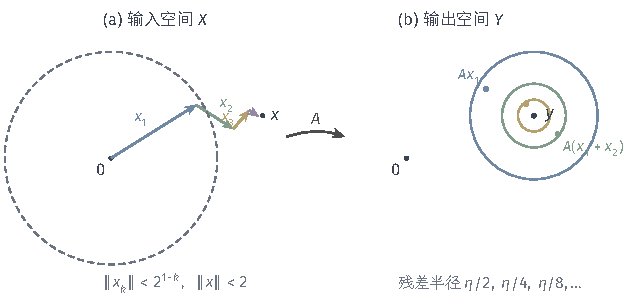
\includegraphics[width=107.4mm]{figures/02-abstract-mathematics/03-function-spaces/tikz/c2-open-mapping/figure.pdf}
  \caption{开映射定理证明中的残差修正（示意）。(b)~输出空间中，第一次近似$Ax_1$落在以$y$为心、半径$\eta/2$的球内（蓝圈），加上修正$x_2$后$A(x_1+x_2)$落入半径$\eta/4$的球（绿圈），依此类推；(a)~输入空间中修正量满足$\|x_k\|<2^{1-k}$，部分和收敛到原像$x$，$\|x\|<2$（虚线圆）。输入空间的完备性保证这一级数有极限。}
  \label{fig:lfo-open-mapping}
\end{figure}

\paragraph{由开映射推出有界逆}
设$A$是Banach空间之间的有界双射。由开映射定理，每个$y$有原像$x$满足$\|x\|\leq\delta^{-1}\|y\|$；单射使这个原像就是$A^{-1}y$，所以$\|A^{-1}y\|\leq\delta^{-1}\|y\|$，$A^{-1}$有界。这证明了定理~\ref{thm:lfo-bounded-inverse}。

\paragraph{等价范数}
有界逆定理的一个直接用途是比较范数。设线性空间$X$在两个范数$\|\cdot\|_a$、$\|\cdot\|_b$下都完备，且$\|x\|_a\leq C\|x\|_b$。则单位映射$I:(X,\|\cdot\|_b)\to(X,\|\cdot\|_a)$是有界双射，其逆也有界，于是存在$C'$使$\|x\|_b\leq C'\|x\|_a$：两个范数等价。若两个完备范数之间只有一个方向的控制，另一个方向的控制会自动出现。

\paragraph{像闭合与下有界}
有界逆定理还给出像闭合的判别。设$X,Y$是Banach空间，$A\in\mathcal B(X,Y)$单射。若$\operatorname{Ran}A$闭，则它是Banach空间，$A:X\to\operatorname{Ran}A$是有界双射，逆有界，于是存在$c>0$使
\begin{equation}
 \|Ax\|\geq c\|x\|\qquad(x\in X),
 \label{eq:lfo-bounded-below}
\end{equation}
这时称$A$\term{下有界}（bounded below）。反过来，若$A$下有界，第~\ref{sec:lfo-self-adjoint}节的论证说明$\operatorname{Ran}A$闭。所以对Banach空间之间的有界单射，像闭合当且仅当下有界。$A(x_n)=(x_n/n)$不满足式~\eqref{eq:lfo-bounded-below}，$\|Ae_n\|=1/n$，它的像也确实不闭。第~\ref{sec:ose-first-kind}节将看到，紧算子在无限维中永远不是下有界的，这正是第一类积分方程不稳定的根源。

\subsection{闭图与图范数（补充）}
\label{sec:lfo-closed-graph}

\paragraph{用极限检验连续性}
直接估计$\|Ax\|\leq C\|x\|$有时很困难。另一种思路是只检验一个较弱的条件：若输入$x_n\to x$，并且输出$Ax_n$也收敛到某个$y$，那么$y$是否必定等于$Ax$？这个条件只涉及输入、输出同时收敛的序列，不要求先证明输出收敛。把它写成几何语言：算子的图
\[
 \mathcal G(A)=\{(x,Ax):x\in D(A)\}\subset X\times Y
\]
在乘积范数$\|(x,y)\|=\|x\|+\|y\|$下是闭集。$X,Y$都完备时，$X\times Y$也是Banach空间。\term{闭图定理}（closed graph theorem）说明，对定义在整个完备空间上的算子，这个较弱的条件已经足够。

\begin{theorem}[闭图定理]
\label{thm:lfo-closed-graph}
设$X,Y$是Banach空间，$A:X\to Y$是定义在整个$X$上的线性算子。则$A$有界当且仅当$\mathcal G(A)$在$X\times Y$中闭。
\end{theorem}

\begin{proof}
若$A$有界，$x_n\to x$推出$Ax_n\to Ax$，所以$Ax_n\to y$时$y=Ax$，图闭。

反过来，设图闭。它是Banach空间$X\times Y$的闭线性子空间，因而本身是Banach空间。第一坐标投影$\pi(x,Ax)=x$是从$\mathcal G(A)$到$X$的有界线性双射（$\|x\|\leq\|(x,Ax)\|$；双射是因为$A$定义在整个$X$上，每个$x$恰好对应图中一点）。由有界逆定理，$\pi^{-1}$有界：存在$C$使$\|x\|+\|Ax\|\leq C\|x\|$，于是$\|Ax\|\leq C\|x\|$。
\end{proof}

\paragraph{处处有定义的对称算子有界}
闭图定理的一个漂亮应用：设$A:H\to H$是定义在整个Hilbert空间上的线性算子，且$\langle v,Au\rangle=\langle Av,u\rangle$对一切$u,v$成立，则$A$有界。只需验证图闭：若$u_n\to u$且$Au_n\to w$，则对任意$v$，
\[
 \langle v,w\rangle=\lim_n\langle v,Au_n\rangle=\lim_n\langle Av,u_n\rangle=\langle Av,u\rangle=\langle v,Au\rangle ,
\]
所以$w=Au$。这里没有估计任何范数，只用了对称性和内积的连续性。反过来说，无界的对称算子（例如适当定义域上的微分算子）不可能定义在整个Hilbert空间上。

\paragraph{定义域只是子空间时}
定理要求$A$定义在整个$X$上。若$A$只定义在子空间$D(A)\subset X$上，图闭合不再意味着有界。回到第~\ref{sec:lfo-boundedness}节的求导$D:D(D)=C^1([0,2\pi])\subset C([0,2\pi])\to C([0,2\pi])$。它的图是闭的：若$u_n\to u$且$u_n'\to v$都按一致范数，则由
\[
 u_n(x)=u_n(0)+\int_0^xu_n'(t)\,dt
\]
两边取极限（一致收敛允许在积分号下取极限）得$u(x)=u(0)+\int_0^xv(t)\,dt$，所以$u\in C^1$且$u'=v$。可是我们已经用$\sin(nx)$说明$D$在一致范数下无界。两者并不矛盾：$D(D)=C^1([0,2\pi])$在一致范数下不完备，闭图定理的条件不满足。图闭合的算子称为\term{闭算子}（closed operator）。

\paragraph{图范数使定义域完备}
对闭算子$A$，在定义域上换用\term{图范数}（graph norm）
\[
 \|u\|_A=\|u\|_X+\|Au\|_Y .
\]
$(D(A),\|\cdot\|_A)$与图$\mathcal G(A)$等距，图闭意味着它完备，而$\|Au\|_Y\leq\|u\|_A$说明$A$在新范数下有界。对求导，图范数正是$\|u\|_\infty+\|u'\|_\infty=\|u\|_{C^1}$，这就回到了第~\ref{sec:lfo-boundedness}节的结论：同一个作用规则，在计入导数的范数下是有界算子。第~\ref{chap:weak-derivatives-sobolev}章的Sobolev范数沿用了同样的思想，用积分范数同时控制函数和它的弱导数。

无界闭算子的谱、由它们生成的算子半群以及相应的演化方程，属于动力系统与轨迹演化问题，可参考\BookChapterRef{chap:action-and-state}{卷三“动力系统”章}。
